\documentclass[11pt, a4paper]{article}
%\usepackage{proj1}
\usepackage{natbib}
\usepackage{fancyhdr}  
\usepackage{subcaption}
\usepackage{caption}
\usepackage{graphicx}
\usepackage{numprint}
\usepackage{multirow}
\linespread{1.25} 
\setlength{\parindent}{0cm}
\graphicspath{{Images/}}
\usepackage{hyperref}
\usepackage{amsmath}
\usepackage{amsfonts}
\usepackage{amssymb}
\usepackage{amsthm}
\usepackage{mathtools}
\usepackage{commath}
\usepackage{bbm}

%\usepackage[sc,osf]{mathpazo}
\usepackage{subcaption}
\usepackage[a4paper, top=1in, left=1.0in, right=1.0in, bottom=1in, includehead, includefoot]{geometry} %Usually have top as 1in

\usepackage{listings}
\usepackage{color} %red, green, blue, yellow, cyan, magenta, black, white
\definecolor{mygreen}{RGB}{28,172,0} % color values Red, Green, Blue
\definecolor{mylilas}{RGB}{170,55,241}


\hypersetup{colorlinks,linkcolor={black},citecolor={blue},urlcolor={black}}
\usepackage{color}
\urlstyle{same}


\theoremstyle{definition}
\newtheorem{definition}{Definition}[section]

%\newcommand{\Sta}{\rho}
\newcommand{\Adj}{p}
\newcommand{\adj}{q}
%\newcommand{\Con}{u}
\newcommand{\Sta}{\rho}
\newcommand{\Stav}{\mathbf{v}}
\newcommand{\Adja}{\mathbf{p}}
\newcommand{\Adjb}{q}
\newcommand{\Adjc}{{p}_{\partial \Sigma}}
\newcommand{\Con}{\mathbf{f}}
\newcommand{\nor}{\mathbf{n}}




\pagenumbering{gobble}
\begin{document}
	\section*{Report 19/08/2020}
	\section{Testing AD Exact/ dissecting domains/ etc -- Forward}
	Testing the exact solution for AD on an infinite domain. It works well on domain in Figure \ref{FD1}. Errors are small and decrease with increasing number of points.
	\begin{align*}
	&N = 20 \quad Abs = 0.00015915 \quad Rel = 1.2555 \times 10^{-7}\\
	&N = 30 \quad Abs = 1.1279 \times 10^{-6} \quad Rel = 1.1311 \times 10^{-9}\\
	&N = 40 \quad Abs = 1.1141 \times 10^{-6} \quad Rel = 1.1173 \times 10^{-9}.\\
	\end{align*}
	
	\begin{figure}[h]
		\centering
		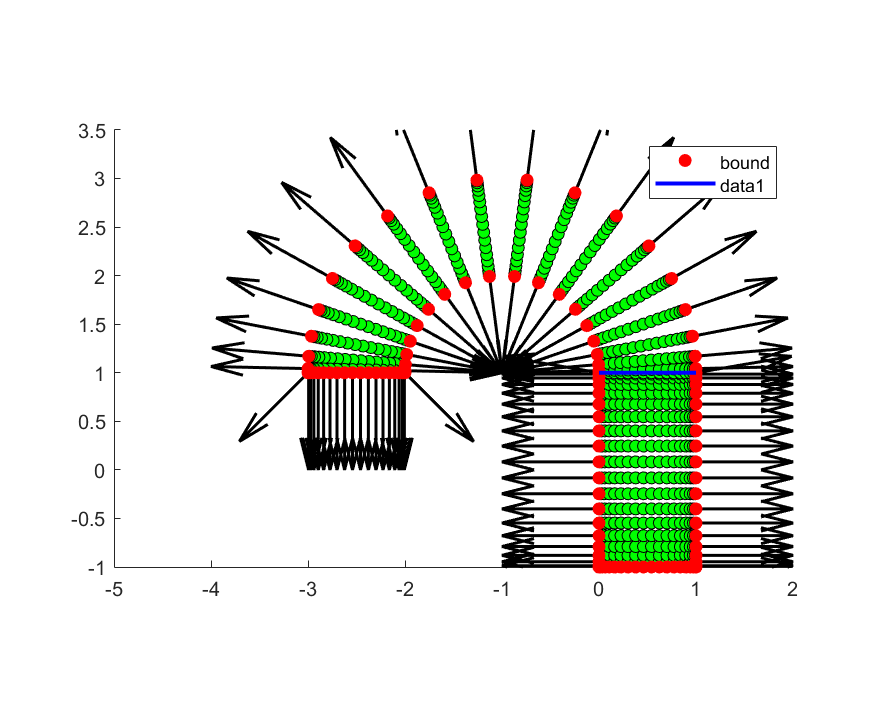
\includegraphics[scale=0.5]{D1.png}
		\caption{Domain1} 
		\label{FD1}
	\end{figure}
	\begin{figure}[h]
		\centering
		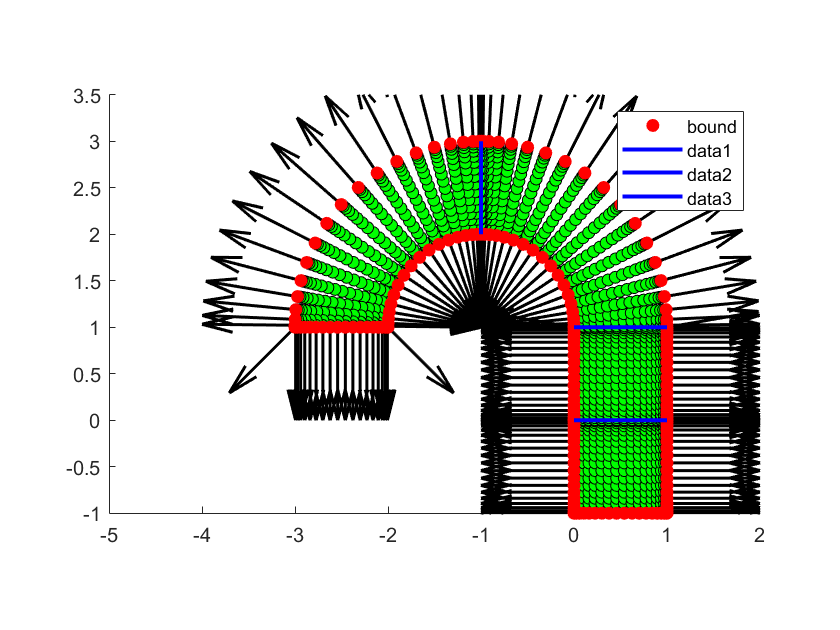
\includegraphics[scale=0.5]{D1a.png}
		\caption{Domain1 dissected} 
		\label{FD1a}
	\end{figure}
   When dissecting the two shapes into two sub-shapes each, the domain is like in Figure \ref{FD1a}.
   Running the problem with $N = 20$, the solution looks the same to the above and gives the errors:
   \begin{align*}
   	&N = 20 \quad Abs = 1.6234\times 10^{-6} \quad Rel = 1.1511 \times 10^{-9}.\\
   \end{align*}
   Running the 'CompareAll' function on the dissected domain gives errors as in screenshot Figure \ref{FS}.
   \begin{figure}[h]
   	\centering
   	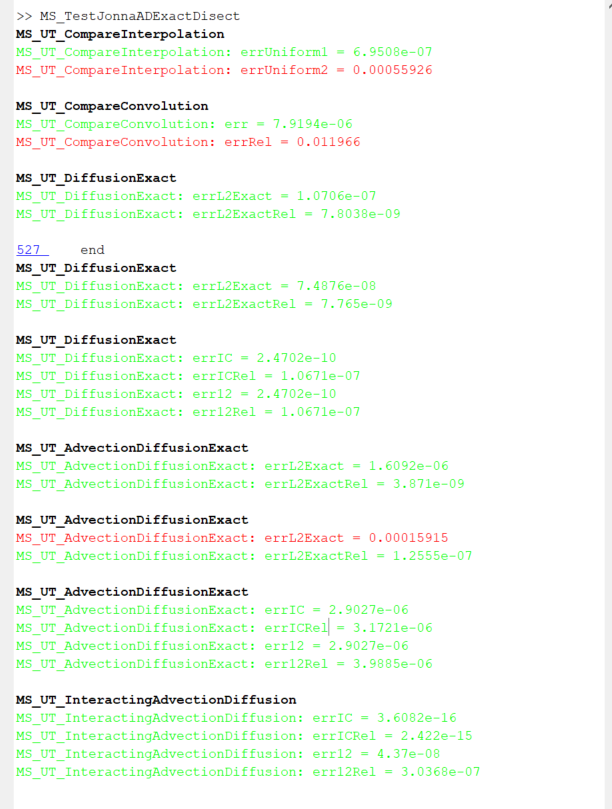
\includegraphics[scale=0.8]{Errors.png}
   	\caption{Errors dissected} 
   	\label{FS}
   \end{figure}
   The only potential point of concern is the interpolation error, see Figure \ref{FInterpE}. We get errors of up to $10^{-4}$. However, I think overall it is ok. I think it may be that $20$ points on only two shapes are not enough but on four shapes they are. When rerunning interpolation with $N = 30$, the error decreases to $10^{-6}$.
    \begin{figure}[h]
   	\centering
   	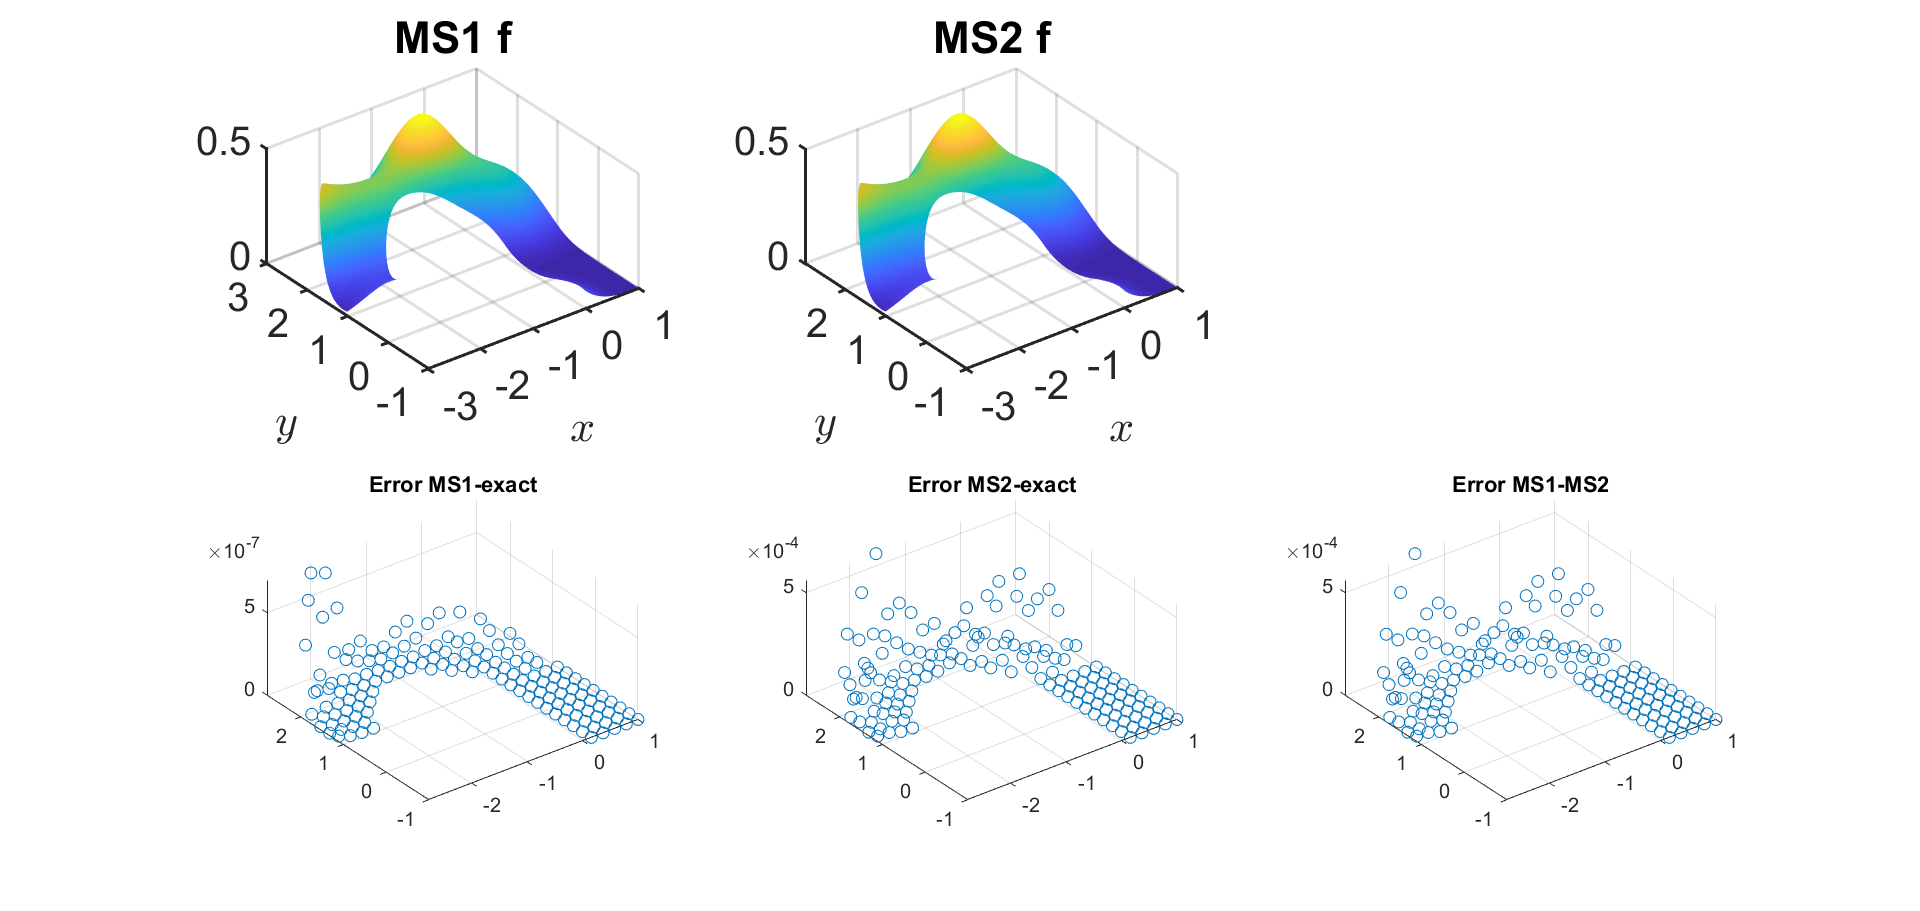
\includegraphics[scale=0.3]{InterpE.png}
   	\caption{Interpolation Errors} 
   	\label{FInterpE}
   \end{figure}
   Out of interest, I ran the exact solution on a larger domain, see Figure \ref{FD3}. The errors are essentially the same as the ones without the extra shape. However, most of the particle mass is in the first two shapes anyway, so I am not quite sure if this is the best test.
   \begin{figure}[h]
   	\centering
   	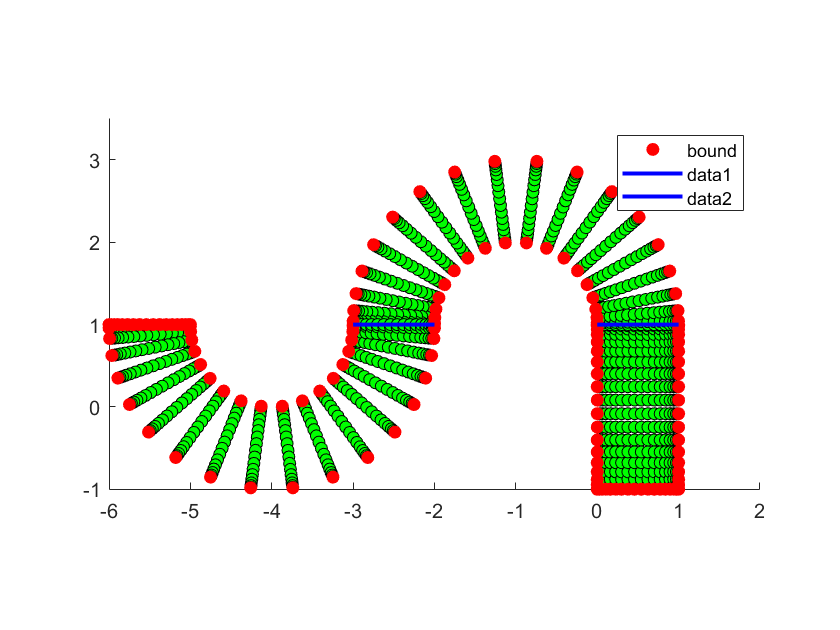
\includegraphics[scale=0.3]{D3.png}
   	\caption{Domain3} 
   	\label{FD3}
   \end{figure}

\section{AD Not Exact}
Tested two different problems with an advection-diffusion no-flux problem. Example 1 is made of 4 shapes and the problem is solved without interactions present.
The advection vector is just constant in the `direction of the shape' and of strength $10$. The initial condition is:$exp(-2((y1 - 0.5 )^2 + (y2 + 1)^2))$. The dynamics is in Figure \ref{FDyn1}.
   \begin{figure}[h]
	\centering
	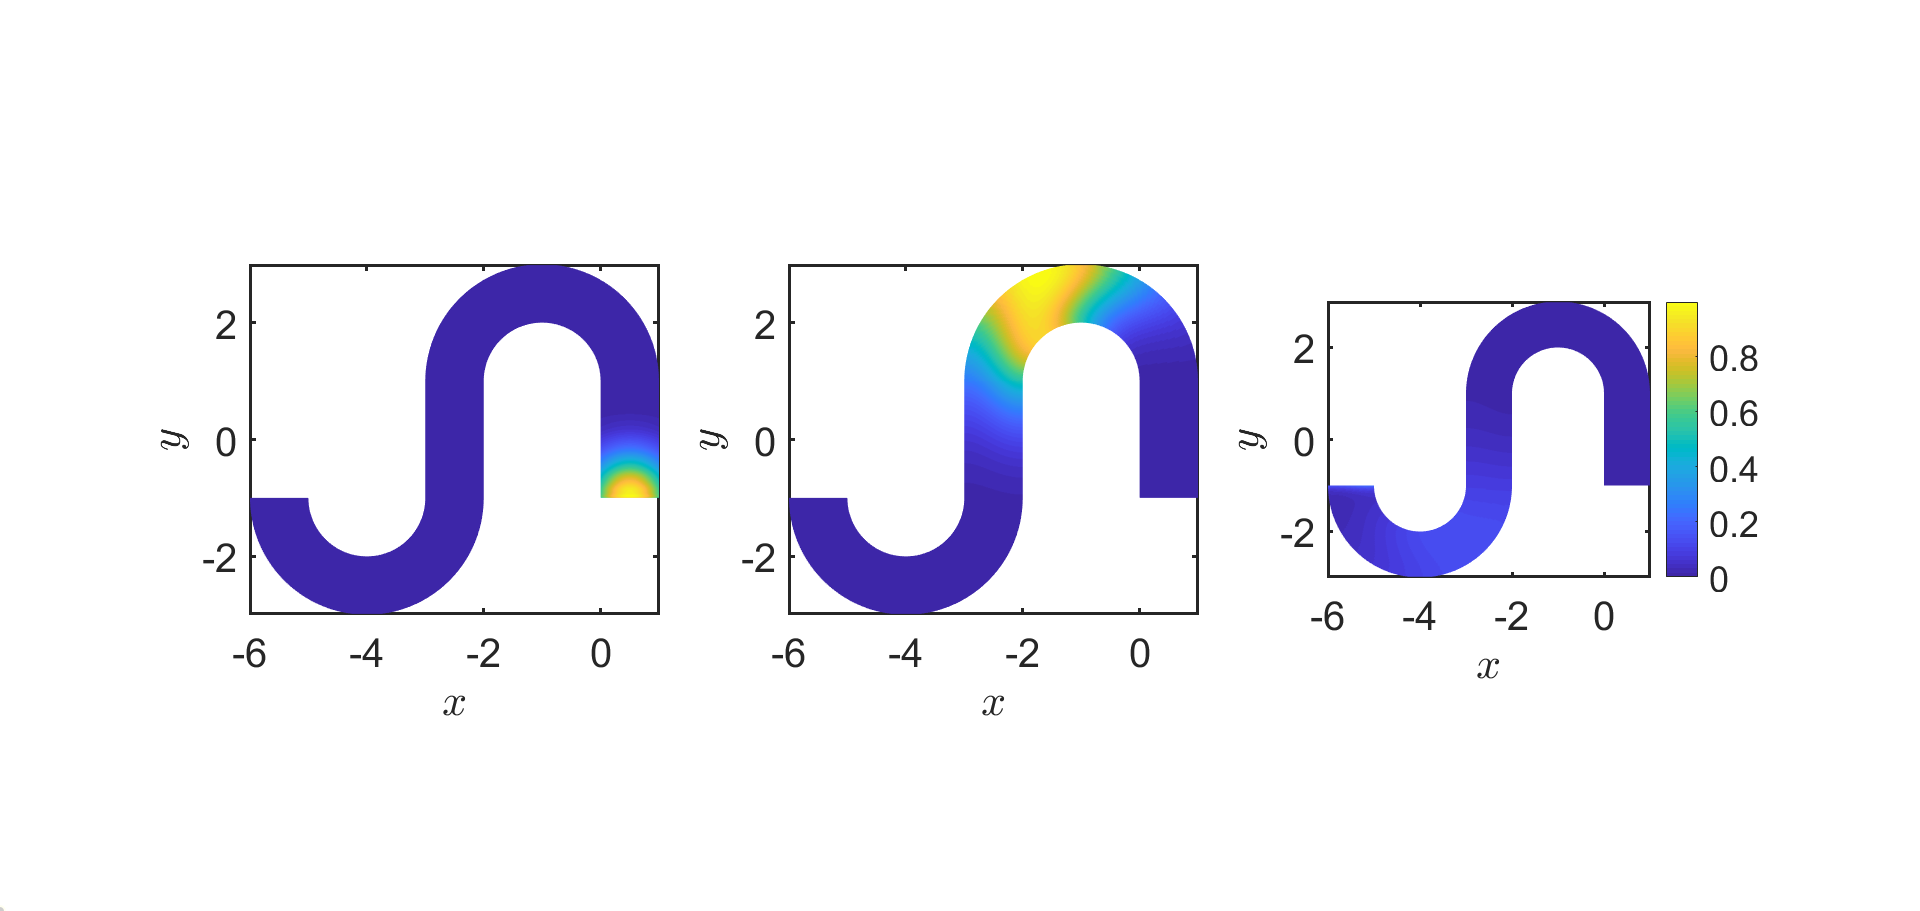
\includegraphics[scale=0.35]{Dyn1.png}
	\caption{Dynamics 1} 
	\label{FDyn1}
\end{figure}
In the second problem we add interaction and a no-flux wall. We have three shapes. The initial condition is: $exp(-2((y1 - 0.8)^2 + (y2 -0.2)^2))$. The result for $\kappa = 1$ is in Figure \ref{FDyn2k1}. The result for $\kappa = - 1$ is in Figure \ref{FDyn2kn1}. The differences are not very visible, however the two figures do show slightly different profiles for $\rho$.
   \begin{figure}[h]
	\centering
	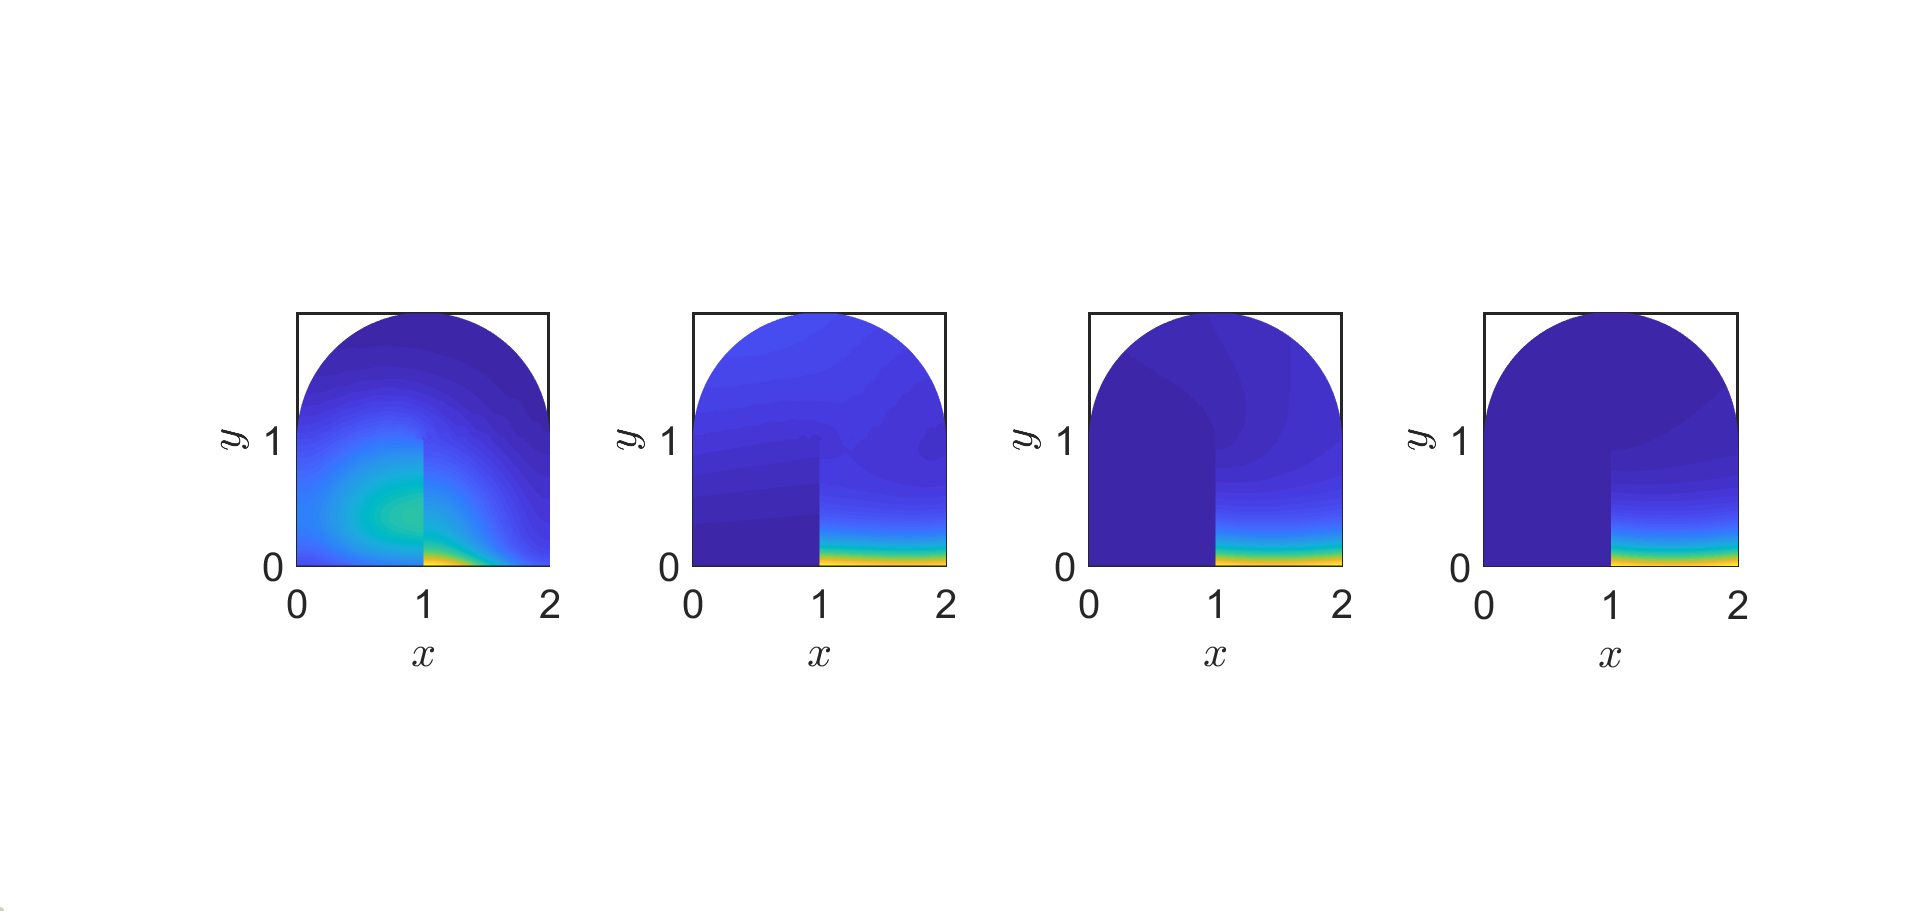
\includegraphics[scale=0.35]{Dyn2k1.png}
	\caption{Dynamics 2 $\kappa = 1$, over time} 
	\label{FDyn2k1}
\end{figure}
   \begin{figure}[h]
	\centering
	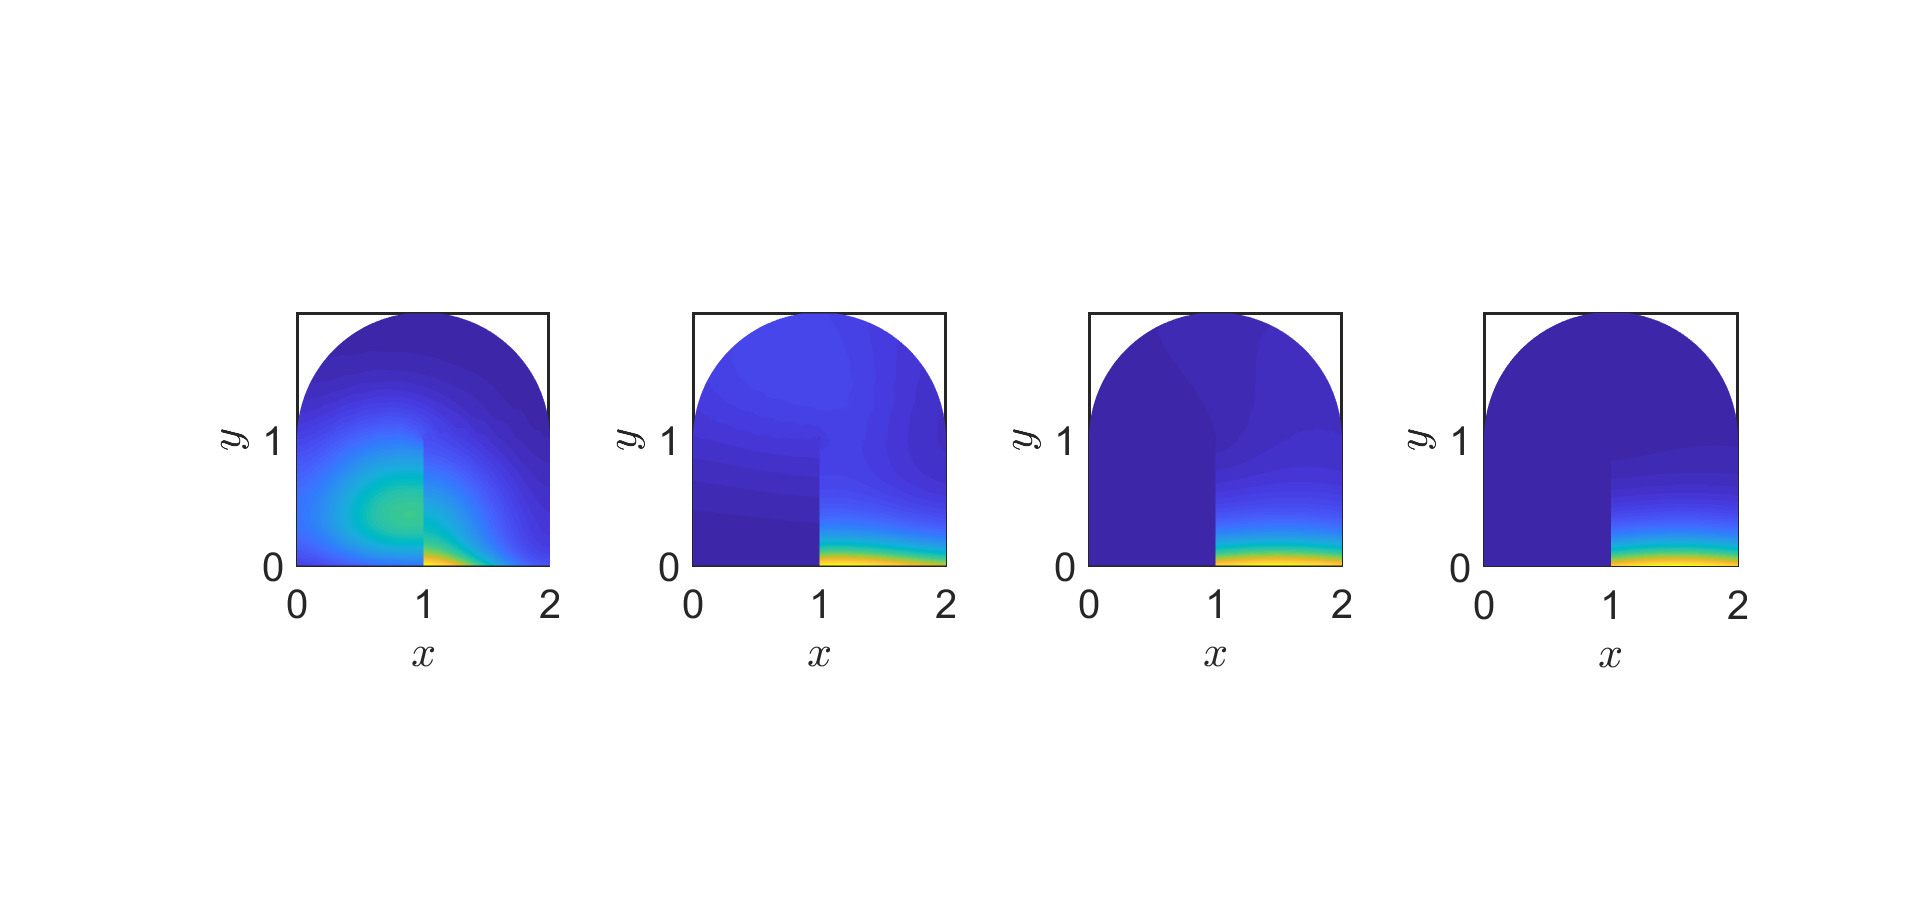
\includegraphics[scale=0.35]{Dyn2kn1.png}
	\caption{Dynamics 2 $\kappa = -1$, over time} 
	\label{FDyn2kn1}
\end{figure}

\section{Migrating to PDECO}
Started migrating the code to PDECO framework.
A few problems arise:\\
- No 'ComputeAll' function for MS. Therefore rewrote Computation but probably not the best way of fixing this.\\
- Preprocessing in PDECO is not compartible with MS because inputs don't match. Changed it in Multishape but that probably isn't working for directly making the shape.\\
- There's a problem with DataStorage and multiple shapes. It can take one rectangular quadrilateral though.\\
\\
Tested with a box made by MS code and Box code. Tested this with both exact AD on infinite domain and on exact solution for Neumann Flow.\\
Tested two boxes that make our standard domain with ADInf. Tested box and wedge with ADInf.\\
Compared the solution to normal box by plotting. It's the same\\
All errors with respect to the exact solution are of order $10^{-9}$ or $10^{-8}$. Errors on the same domain for the two different shape classes are $10^{-13}$ for $rhoNum$.\\
can run a simple AD problem like above. with constant velocity profile (See figure 6 for example). Checked no flux boundary between two shapes too.\\
\\
\\
Started implementing the optimization aspect. Works for box shaped MS code and Neumann Flow Exact problem.\\
Tried to split box and still use Neumann Flow Exact. Doesn't work because the error in the adjoint is too large -- why? Plotting it, the two adjoints look very similar.\\
Started a random problem with constant flow on square+wedge, with constant flow. It runs but is slow obviously, so don't know result. 

\end{document}